% Figure 1: running examples; the lower two blocks retain their previous design.
\RequirePackage{fix-cm}
\documentclass[border=0pt]{standalone}
\usepackage[T1]{fontenc}
\usepackage{times}
\usepackage{amsmath,amssymb}
\usepackage{tikz}
\usetikzlibrary{arrows.meta}
\definecolor{reorg}{HTML}{315F88}
\definecolor{control}{HTML}{286B66}
\begin{document}
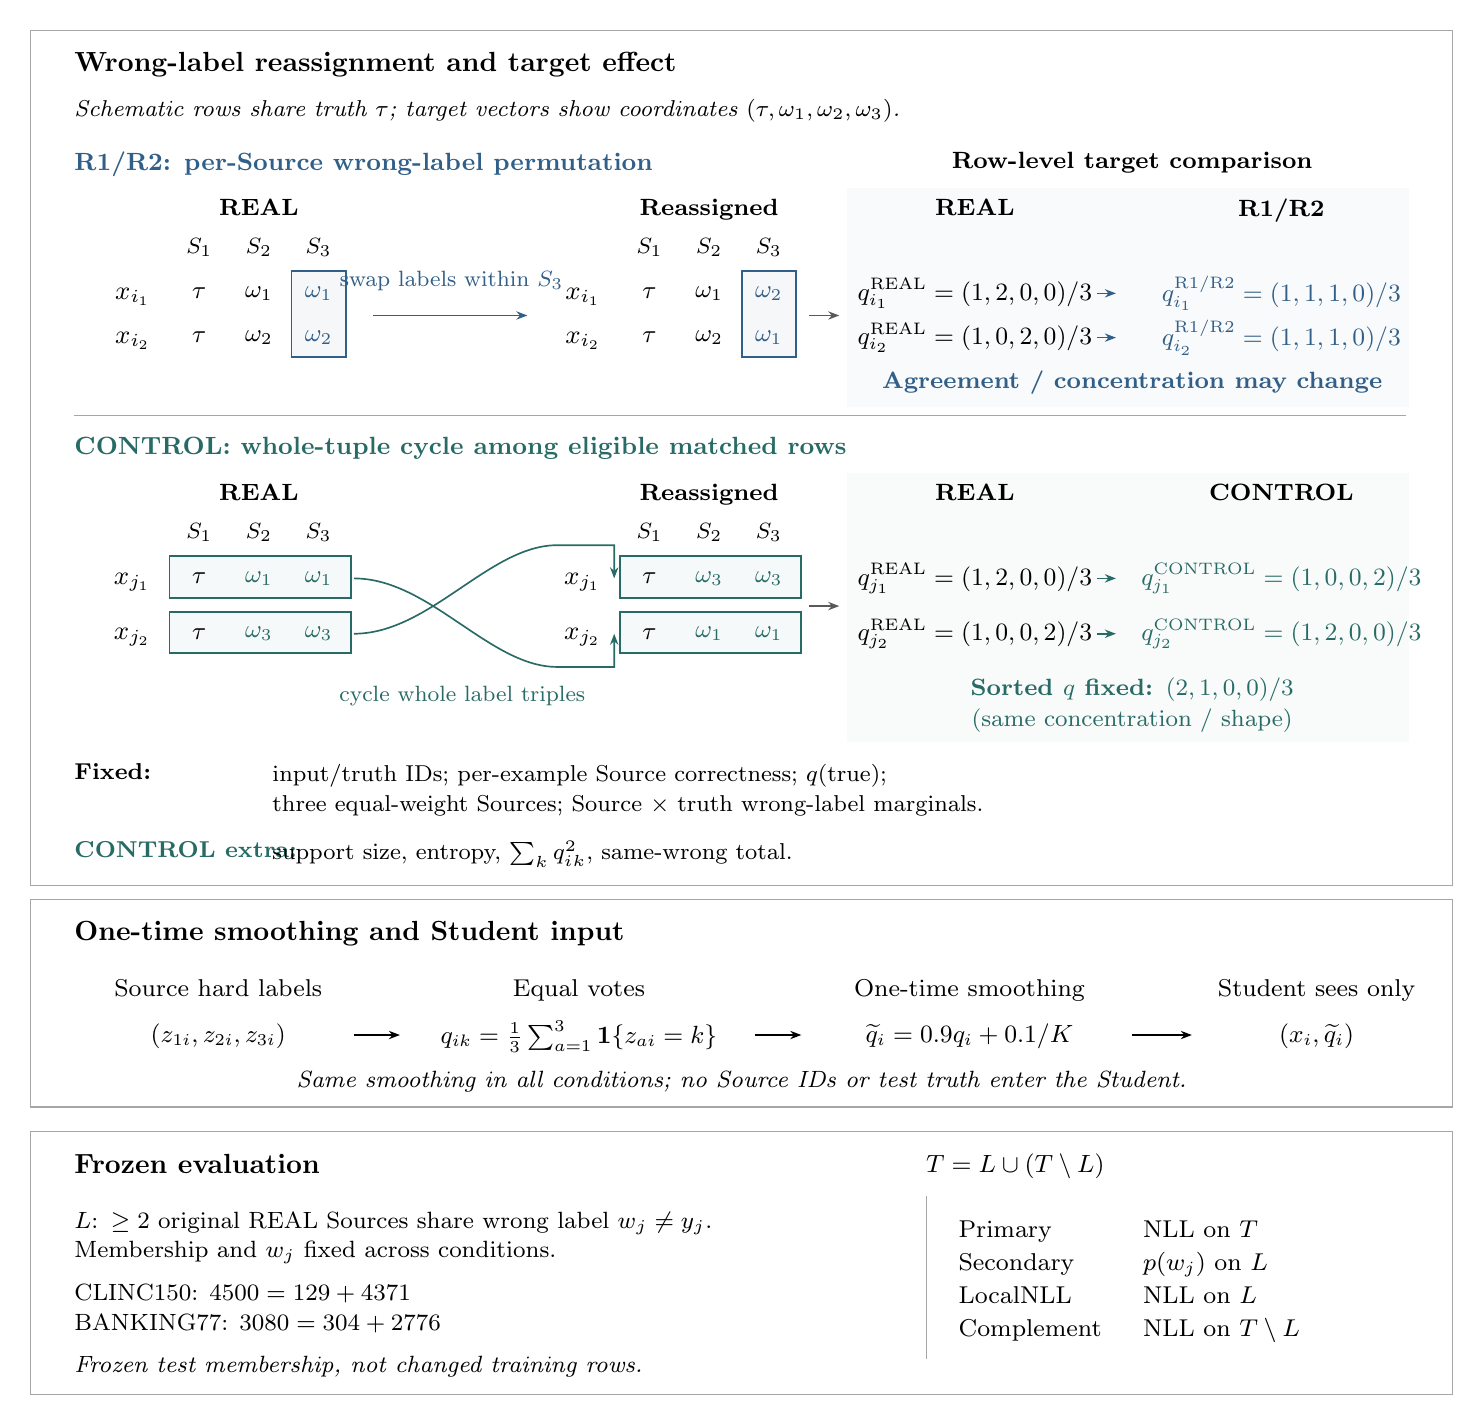
\begin{tikzpicture}[x=1pt,y=-1pt,
  every node/.style={inner sep=0pt,outer sep=0pt,anchor=north west,
    font=\fontsize{9}{11}\selectfont,align=left},
  flow/.style={-{Stealth[length=4pt,width=3pt]},line width=.6pt},
  frame/.style={draw=black!35,line width=.4pt},
  heading/.style={font=\bfseries\fontsize{10}{12}\selectfont}]
\path[use as bounding box] (0,0) rectangle (516,495);
\draw[frame] (1,1) rectangle (515,310);
\draw[frame] (1,315) rectangle (515,390);
\draw[frame] (1,399) rectangle (515,494);
% Coordinate-only inset: node text and fonts are not scaled.
\begin{scope}[xshift=5.16pt,xscale=.98]


\node[heading] at (12,9) {Wrong-label reassignment and target effect};
\node[font=\itshape\fontsize{8.3}{10}\selectfont] at (12,26)
  {Schematic rows share truth $\tau$; target vectors show coordinates $(\tau,\omega_1,\omega_2,\omega_3)$.};

% R1/R2: only S3's wrong labels exchange; the other columns stay fixed.
\node[font=\bfseries\fontsize{9}{11}\selectfont,text=reorg] at (12,45)
  {R1/R2: per-Source wrong-label permutation};
\node[anchor=north,font=\bfseries\fontsize{8.5}{10}\selectfont] at (402,45) {Row-level target comparison};
\fill[reorg!3] (297,58) rectangle (504,137);
\node[anchor=north,font=\bfseries\fontsize{8.5}{10}\selectfont] at (80,62) {REAL};
\node[anchor=north,font=\bfseries\fontsize{8.5}{10}\selectfont] at (246,62) {Reassigned};
\node[anchor=north,font=\bfseries\fontsize{8.5}{10}\selectfont] at (344,62) {REAL};
\node[anchor=north,font=\bfseries\fontsize{8.5}{10}\selectfont] at (457,62) {R1/R2};
\foreach \x/\s in {58/1,80/2,102/3,224/1,246/2,268/3}{
  \node[anchor=north,font=\fontsize{8}{9}\selectfont] at (\x,76) {$S_{\s}$};
}
% Correct tau cells stay unfilled; wrong-label reassignment carries the accent.
\foreach \x in {102,268}{\draw[reorg,line width=.65pt,fill=reorg!5] (\x-10,88) rectangle (\x+10,119);}
\foreach \x in {58,224}{
  \node[anchor=center] at (\x,96) {$\tau$};
  \node[anchor=center] at (\x,112) {$\tau$};
}
\foreach \x in {80,246}{
  \node[anchor=center] at (\x,96) {$\omega_1$};
  \node[anchor=center] at (\x,112) {$\omega_2$};
}
\node[anchor=center,text=reorg] at (102,96) {$\omega_1$};
\node[anchor=center,text=reorg] at (102,112) {$\omega_2$};
\node[anchor=center,text=reorg] at (268,96) {$\omega_2$};
\node[anchor=center,text=reorg] at (268,112) {$\omega_1$};
\foreach \x in {40,206}{
  \node[anchor=mid east,font=\fontsize{9.5}{11}\selectfont] at (\x,96) {$x_{i_1}$};
  \node[anchor=mid east,font=\fontsize{9.5}{11}\selectfont] at (\x,112) {$x_{i_2}$};
}
\draw[flow,reorg] (122,104)--(179,104);
\node[anchor=north,font=\fontsize{8}{9}\selectfont,text=reorg] at (151,88) {swap labels within $S_3$};
\draw[flow,black!65] (283,104)--(294,104);
\node[anchor=center] at (344,96) {$q^{\mathrm{REAL}}_{i_1}=(1,2,0,0)/3$};
\node[anchor=center] at (344,112) {$q^{\mathrm{REAL}}_{i_2}=(1,0,2,0)/3$};
\node[anchor=center,text=reorg] at (457,96) {$q^{\mathrm{R1/R2}}_{i_1}=(1,1,1,0)/3$};
\node[anchor=center,text=reorg] at (457,112) {$q^{\mathrm{R1/R2}}_{i_2}=(1,1,1,0)/3$};
\draw[flow,reorg] (389,96)--(396,96);
\draw[flow,reorg] (389,112)--(396,112);
\node[anchor=north,font=\bfseries\fontsize{8.5}{10}\selectfont,text=reorg] at (402,124)
  {Agreement / concentration may change};

% CONTROL: matched, eligible rows; arrows attach to whole tuple boundaries.
\draw[frame] (12,140)--(503,140);
\node[font=\bfseries\fontsize{9}{11}\selectfont,text=control] at (12,148)
  {CONTROL: whole-tuple cycle among eligible matched rows};
\fill[control!3] (297,161) rectangle (504,258);
\node[anchor=north,font=\bfseries\fontsize{8.5}{10}\selectfont] at (80,165) {REAL};
\node[anchor=north,font=\bfseries\fontsize{8.5}{10}\selectfont] at (246,165) {Reassigned};
\node[anchor=north,font=\bfseries\fontsize{8.5}{10}\selectfont] at (344,165) {REAL};
\node[anchor=north,font=\bfseries\fontsize{8.5}{10}\selectfont] at (457,165) {CONTROL};
\foreach \x/\s in {58/1,80/2,102/3,224/1,246/2,268/3}{
  \node[anchor=north,font=\fontsize{8}{9}\selectfont] at (\x,179) {$S_{\s}$};
}
\foreach \x in {47,213}{
  \draw[control,line width=.65pt,fill=control!4] (\x,191) rectangle (\x+67,206);
  \draw[control,line width=.65pt,fill=control!4] (\x,211) rectangle (\x+67,226);
}
\foreach \x in {58,224}{
  \node[anchor=center] at (\x,199) {$\tau$};
  \node[anchor=center] at (\x,219) {$\tau$};
}
\foreach \x in {80,102}{
  \node[anchor=center,text=control] at (\x,199) {$\omega_1$};
  \node[anchor=center,text=control] at (\x,219) {$\omega_3$};
}
\foreach \x in {246,268}{
  \node[anchor=center,text=control] at (\x,199) {$\omega_3$};
  \node[anchor=center,text=control] at (\x,219) {$\omega_1$};
}
\foreach \x in {40,206}{
  \node[anchor=mid east,font=\fontsize{9.5}{11}\selectfont] at (\x,199) {$x_{j_1}$};
  \node[anchor=mid east,font=\fontsize{9.5}{11}\selectfont] at (\x,219) {$x_{j_2}$};
}
% Curved crossed transfers show j1 -> j2 and j2 -> j1, including S1.
\draw[flow,control] (115,199) .. controls (143,199) and (165,231) .. (190,231)
  --(211,231)--(211,219);
\draw[flow,control] (115,219) .. controls (143,219) and (165,187) .. (190,187)
  --(211,187)--(211,199);
\node[anchor=north,font=\fontsize{8}{9}\selectfont,text=control] at (155,238)
  {cycle whole label triples};
\draw[flow,black!65] (283,209)--(294,209);
\node[anchor=center] at (344,199) {$q^{\mathrm{REAL}}_{j_1}=(1,2,0,0)/3$};
\node[anchor=center] at (344,219) {$q^{\mathrm{REAL}}_{j_2}=(1,0,0,2)/3$};
\node[anchor=center,text=control] at (457,199) {$q^{\mathrm{CONTROL}}_{j_1}=(1,0,0,2)/3$};
\node[anchor=center,text=control] at (457,219) {$q^{\mathrm{CONTROL}}_{j_2}=(1,2,0,0)/3$};
\draw[flow,control] (389,199)--(396,199);
\draw[flow,control] (389,219)--(396,219);
\node[anchor=north,font=\bfseries\fontsize{8.5}{11}\selectfont,text=control,align=center] at (402,235)
  {Sorted $q$ fixed: $(2,1,0,0)/3$\\
   \normalfont\fontsize{8.5}{11}\selectfont (same concentration / shape)};

% Two distinct constraint rows; hanging alignment keeps the labels separate.
\node[font=\bfseries\fontsize{8.3}{11}\selectfont] at (12,266) {Fixed:};
\node[font=\fontsize{8.3}{11}\selectfont] at (85,266)
  {input/truth IDs; per-example Source correctness; $q(\mathrm{true})$;\\
   three equal-weight Sources; Source $\times$ truth wrong-label marginals.};
\node[font=\bfseries\fontsize{8.3}{11}\selectfont,text=control] at (12,294) {CONTROL extra:};
\node[font=\fontsize{8.3}{11}\selectfont] at (85,294)
  {support size, entropy, $\sum_k q_{ik}^{2}$, same-wrong total.};

% Lower blocks: unchanged conceptual layout, only functional titles.
\begin{scope}[yshift=-119pt]

\node[heading] at (12,204) {One-time smoothing and Student input};
\node[anchor=north,font=\fontsize{8.8}{11}\selectfont] at (65,225) {Source hard labels};
\node[anchor=north] at (65,241) {$(z_{1i},z_{2i},z_{3i})$};
\draw[flow] (115,245)--(132,245);
\node[anchor=north,font=\fontsize{8.8}{11}\selectfont] at (198,225) {Equal votes};
\node[anchor=north] at (198,240) {$q_{ik}=\frac{1}{3}\sum_{a=1}^{3}\mathbf{1}\{z_{ai}=k\}$};
\draw[flow] (263,245)--(280,245);
\node[anchor=north,font=\fontsize{8.8}{11}\selectfont] at (342,225) {One-time smoothing};
\node[anchor=north] at (342,241) {$\widetilde q_i=0.9q_i+0.1/K$};
\draw[flow] (402,245)--(424,245);
\node[anchor=north,font=\fontsize{8.8}{11}\selectfont] at (470,225) {Student sees only};
\node[anchor=north] at (470,241) {$(x_i,\widetilde q_i)$};
\node[anchor=north,font=\itshape\fontsize{8.5}{10}\selectfont] at (258,258)
  {Same smoothing in all conditions; no Source IDs or test truth enter the Student.};

\node[heading] at (12,288) {Frozen evaluation};
\node[anchor=north west] at (326,288) {$T=L\cup(T\setminus L)$};
\node[text width=316pt,font=\fontsize{8.5}{10.5}\selectfont] at (12,309)
  {$L$: $\geq 2$ original REAL Sources share wrong label $w_j\ne y_j$.\\
   Membership and $w_j$ fixed across conditions.};
\node[font=\fontsize{8.5}{11}\selectfont] at (12,335)
  {CLINC150: $4500=129+4371$\\
   BANKING77: $3080=304+2776$};
\node[font=\itshape\fontsize{8.5}{10}\selectfont] at (12,361)
  {Frozen test membership, not changed training rows.};
\draw[frame] (326,303)--(326,362);
\node[font=\fontsize{8.8}{12}\selectfont] at (338,312)
  {Primary\\Secondary\\LocalNLL\\Complement};
\node[font=\fontsize{8.8}{12}\selectfont] at (406,312)
  {NLL on $T$\\$p(w_j)$ on $L$\\NLL on $L$\\NLL on $T\setminus L$};
\end{scope}
\end{scope}
\end{tikzpicture}
\end{document}
